\documentclass[12pt]{article}
\usepackage{amsmath}
\usepackage{amssymb}
\usepackage{graphicx}
\usepackage[margin=1in]{geometry}
\newcommand{\del}{\nabla}
\begin{document}

\title{Kronecker Graphs for Modelling Linguistic Data}
\author{Howon Lee (howonlee)}
\maketitle

\section{Introduction}

An important statistical regularity in language is Zipf's law, which says that given some corpus of natural language, the frequency of any word is inversely proportional to its rank on the frequency table. However remarkable it may be, however, it is not a statement about the structure of language. This is because it holds for corpuses as bags of words which have frequencies, not as linguistic entities which have internal structure. \cite{smallworldlang}

One important language model which is used in many places which incorporates some aspect of linguistic structure, notably without specifying it, is the n-gram, which takes the semi-Markov assumption that the only context needed to reproduce a word is the past $n$ words. This is of interest, because it turns out that thinking of a corpus as a graph of words and the order-one and order-two relations between words, as bigram and trigram models do, reveals many small-world properties in the structuring of words in corpuses.

We want to deal with the problem of using and adapting already existing algorithms for creating small world nets by creating a parsimonious model of language with Kronecker graphs that respects these network properties of words as they currently exist. We aim to use that language model for a part-of-speech tagging task.

\section{Literature Review}

We review MEJ Newman's \emph{Power laws, Pareto Distributions and Zipf's law}\cite{mejpowerlaw}, J. Leskovec and C. Faloutsos's \emph{Scalable Modeling of Real Graphs using Kronecker Multiplication}\cite{kronfit}, and RF Cancho and RV Sole's \emph{The Small World of Human Language}\cite{smallworldlang}.

\subsection{MEJ Newman}

MEJ Newman's paper is a review and introduction to power laws, which are notable for being found in very many domains across nature, and for the behavior of their first and second moments. That is, the average number of inhabitants of a city is on the order of $10^3$, but that doesn't tell you about the existence of Tokyo.

A particular point of interest is the introduction to a possible information-theoretic origin of Zipf's law. MEJ Newman reviews a possible origin of power law phenomena in language due to Miller\cite{gamiller}. Miller's argument goes like this: imagine a monkey typing on a typewriter, delimiting words with some probability and writing a random letter with some uniform probability. Then, this approximates an exponential distribution of frequency of a word $x$ with number of letters $y$. But the number of possible words goes up exponentially with $y$ also, making the distribution of frequencies a combination of exponentials, which is a power law.

This is a simplistic argument, but can be made less simplistic in talking about arbitrary information in bits instead of symbols in a normal alphabet. However, this theory is only compatible with a random typewriter of information with independence of the typing. However, the example of Shannon's entropy game, where one guesses the next word based upon the previous word in a communication, implies that some conditional structure exists in language, since humans can play Shannon's entropy game. \cite{shannon}
. 

A strong point of the paper is its covering most things which were known about the power law phenomena at the time, and being skeptical about the general trend of plotting some distribution, finding a fat tail or fitting a simple least squares model, and declaring that the phenomenon respected a power law: that skepticism is continued in C. Shalzi's paper\cite{cosma}.

\subsection{Leskovec et al}

A possible model of small world graphs is the stochastic Kronecker graph\cite{kronfit}, which is a sample from a distribution over graphs created by drawing a fractal over an adjacency matrix using the Kronecker product operation. The important thing about this model is that it tries to simultaneously fulfill the many observed properties of small world graphs, not just the heavy tail for indegree and outdegree, but also the heavy tail for scree plots, the densification power law, and small diameters, all at the same time.

The novel contribution of this paper is to note that the parameters for that distribution can be fitted with KronFit, a gradient descent algorithm which learns much bigger graphs much faster than previous attempts to fit graphs like the exponential random graph. This is because it uses MCMC to assign node labels and because it uses the sparsity of the small world graph to estimate the likelihood in time linear to the number of edges instead of quadratic to the number of nodes. The number of parameters is determined using a BIC metric.

There are also real interpretations of the Kronecker product process in the structure and creation of graphs. One intuition is that networks are hierarchically organized into communities, which grow recursively, creating miniature copies of themselves. Another interpretation is to say that each node is described by a sequence of categorical features, and the probability of two nodes linking depends on the product of individual attribute similarities, which allows modelling of homophily and heterophily at the same time.

One important point to take into mind is that one suggested usage for the Kronecker fitting algorithm is for compression of graphs. This is important, because whenever we hear "compression" we should smell "machine learning", because any system of compression can be used for prediction, by finding the symbol that compresses best given the history of the data \cite{mlcompression}.

There is another work which notes that local search (viz., decentralized search) cannot efficiently find paths through Kronecker graphs. This is a large lacuna in the claim that Kronecker graphs are an attempt to model every aspect of how small world networks work at once\cite{stochkrongraph}.

\subsection{Cancho et al}

Cancho and Sole's paper talk about the implicit statistical regularities in a small world net made from the co-occurrence network of words in sentences. Instead of talking about syntactic structure in sentences, they investigate the statistical structure of these mere co-occurrences. Why? Four reasons. It's easier to examine link structures automatically, as opposed to syntactic structures. They don't know what types of links there are in the structures of words, but just having the propinquity of words will capture almost every type. They are not interested in all the links, so looking at whole sentences will not be as productive. Long-distance syntactic links imply the existence of lower-distance syntactic links, but not vice versa.

Looking at the graph created in this way, they find small-world properties like high clustering coefficient, small diameter and power law degree distribution. They hypothesize that this leads to words that exist to speed up navigation in this small world, words like "and", "the", "of", "in", which do not contribute meaning but structure to grammar. They also hypothesize that the disfluency caused in agrammatism is caused by disruption to this small world.

\section{Project Status}

\subsection{Problem}

If we take the central thesis of RF Cancho and RF Sole's work to be true, then word networks are small world networks. Therefore, they should be able to be fitted to parameters for a Kronecker distribution, which would compress the language graph to a very few parameters. It should be investigated whether these parameters, this model has any value as a language model.

The problem that this language model should be used in is a part-of-speech tagger and in a generative model. The generative model should be used to generate text, and examined to see if it generates reasonable test. The language model can be fit into a POS tagger as a prior for the optimization target in a noisy channel model.\cite{collins}

\subsection{Data}
We will use the Gutenberg NLTK corpus for the model, splitting it for development and testing. We will also make use of the POS tags from the Penn Treebank, when we implement the full POS system. \cite{nltk}

\subsection{Evaluation}
Perplexity is an easy development measure of the generator's goodness. Of course, it's a bad approximation of anything we care about in the generalization performance. In order to judge mellifluousness, we should evaluate the generated text with human evaluators from Mechanical Turk.

There are well-established methods for evaluation for the POS tagging task, since it is a well-defined machine learning task. Therefore, we will look at accuracy and F1 compared to a gold set from the Penn Treebank, comparing this KronFit tagger to a trigram baseline, a HMM trigram tagger.

\subsection{Preliminary Results}

Because the RF Cancho and RV Sole paper was from 2001, there exist some properties of small world graphs which were first published afterwards and therefore for good reason were not examined. For example, the densification power law\cite{densificationpowerlaw} and skewed network values\cite{netvalskew} are properties reviewed in the Kronecker graph article but not in this paper, among others. So figures 1 and 2 are an analysis of those two properties using a 1st-order word net (bigram). In this case, this is a directed and not an undirected graph. KS test for the densification versus $x^{1.14}$ has $p>0.1$ (we want a big $p$).

\begin{figure}
  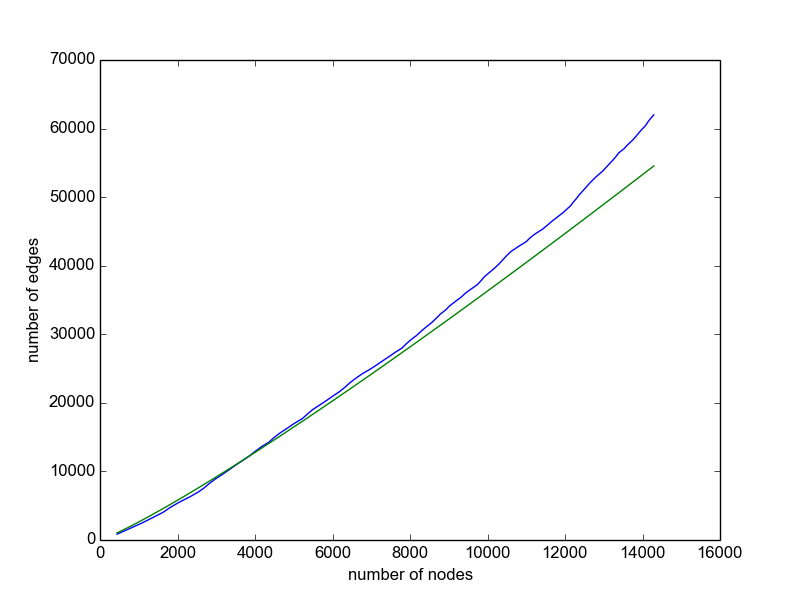
\includegraphics[width=0.45\textwidth]{densification_plot.png}
  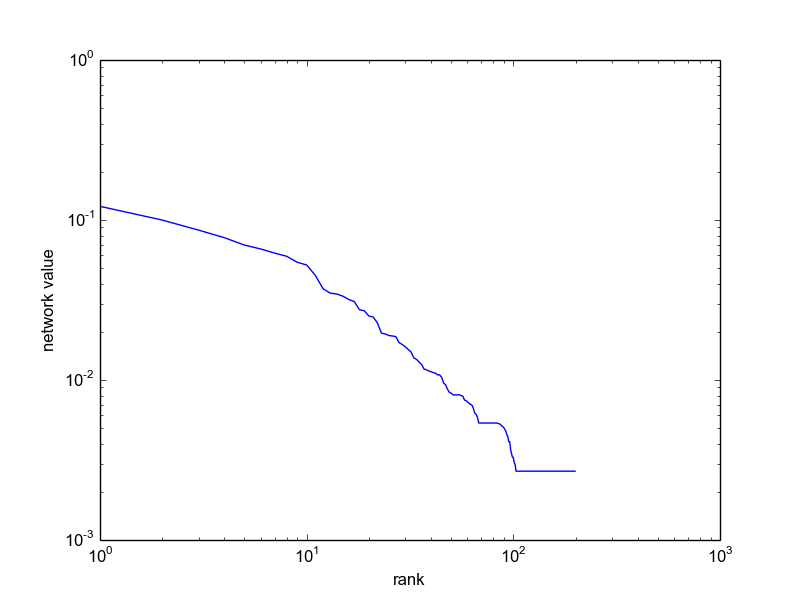
\includegraphics[width=0.45\textwidth]{eigenvector_loglog.png}
  \caption{left: densification plot, with $x^{1.14}$ plotted, right: network value plot}
\end{figure}

We have not made significant progress on the POS tagging system, becaue the generative model will be a component of the POS tagging system only. However, we have made significant progress on the generative model. We have the Kronecker model with 36 (6 by 6) and with 4 parameters(2 by 2), fitted on a bigram model of the corpus construed as a matrix. We chose the number of parameters not according to the principled BIC method but by guessing. In this case, therefore, we are construing KronFit as a way to compress a matrix very well: here, the bigram matrix, later, the trigram matrix.

A significant problem remains the matching of the node labels to the words. Since we had the node label sampling subroutine in the snap library, a simple heuristic was taking the last sample after the whole chain had run, reasoning that that would be from something like the stationary distribution of node labels. It is, but it is still a single sample.
\begin{figure}
  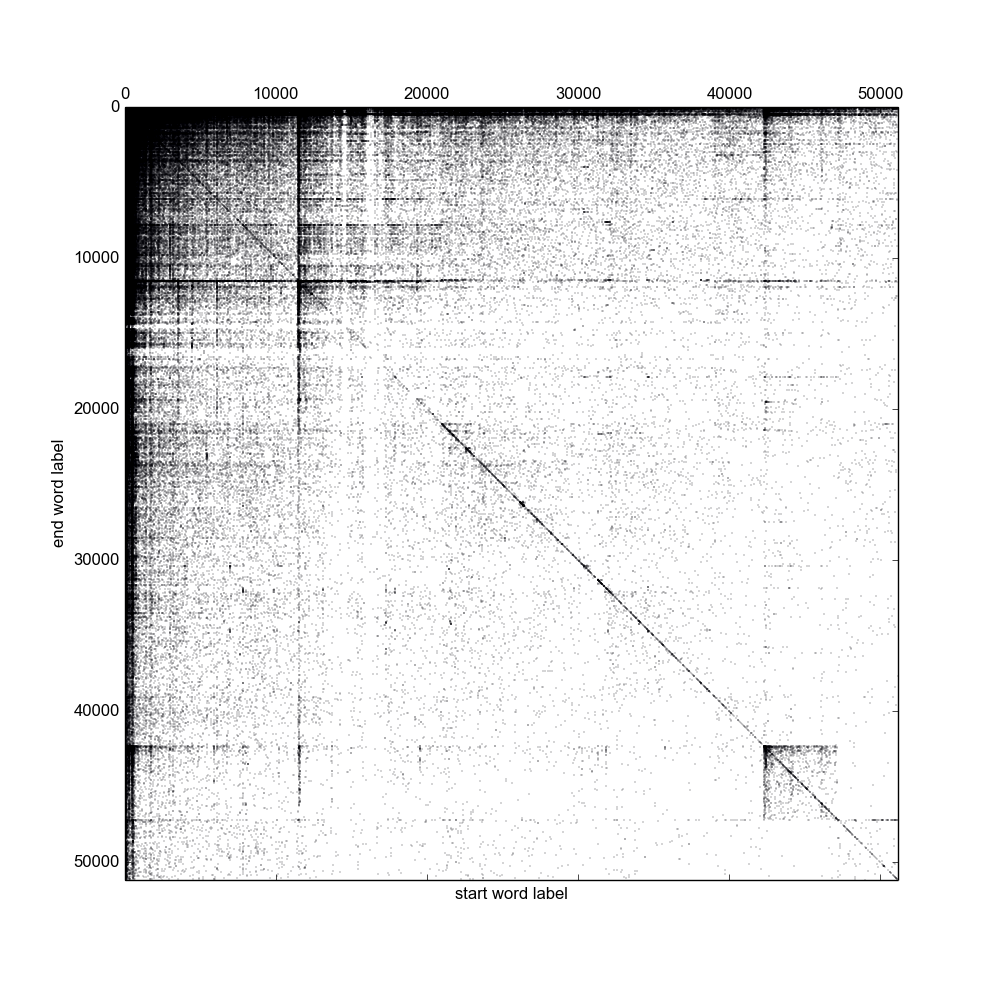
\includegraphics[width=0.45\textwidth]{bigram_sparsematplot.png}
  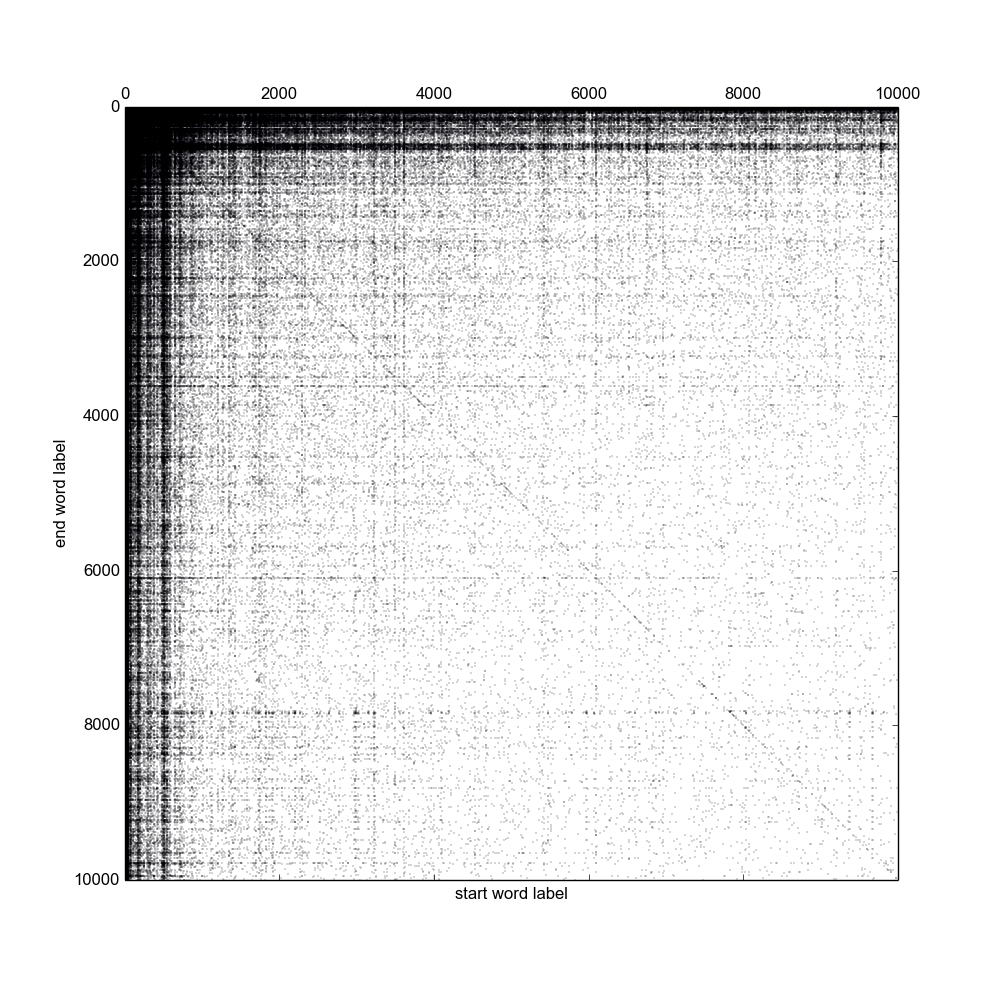
\includegraphics[width=0.45\textwidth]{bigram_small_sparsematplot.png}
  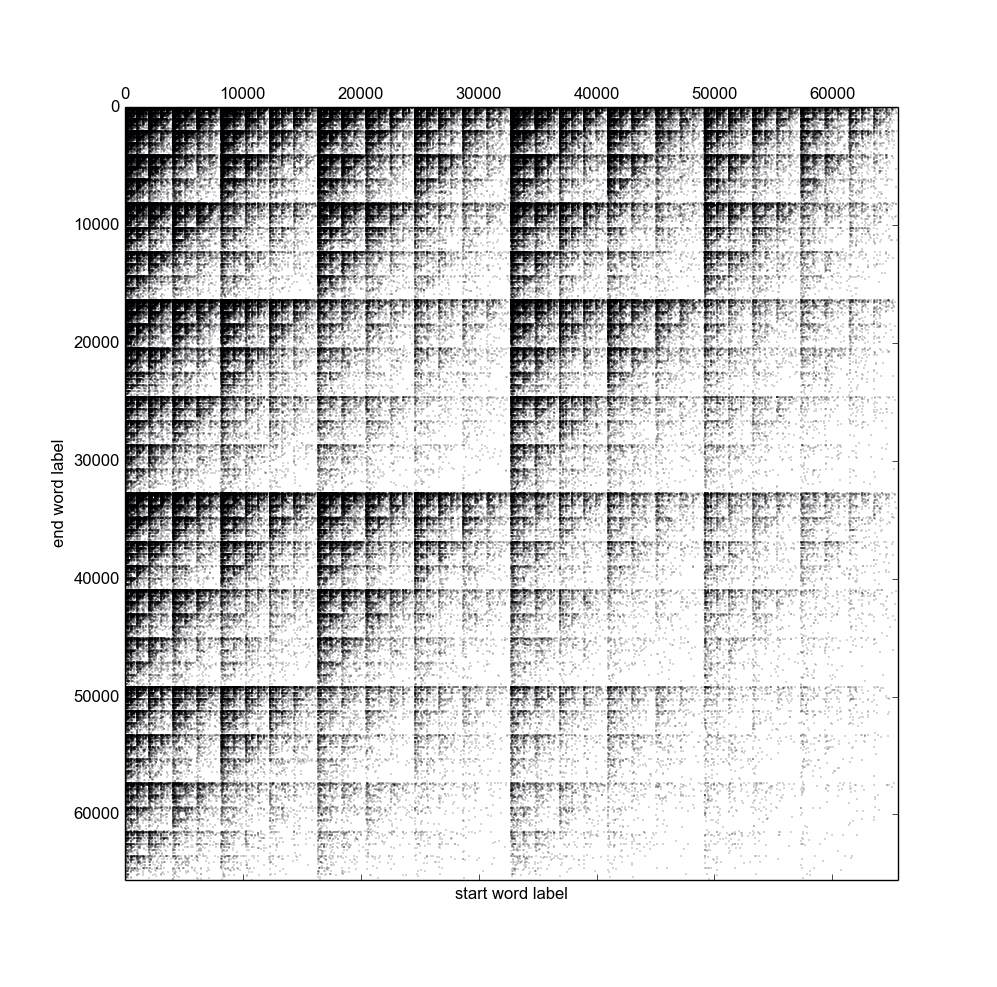
\includegraphics[width=0.45\textwidth]{kronfit2_sparsematplot.png}
  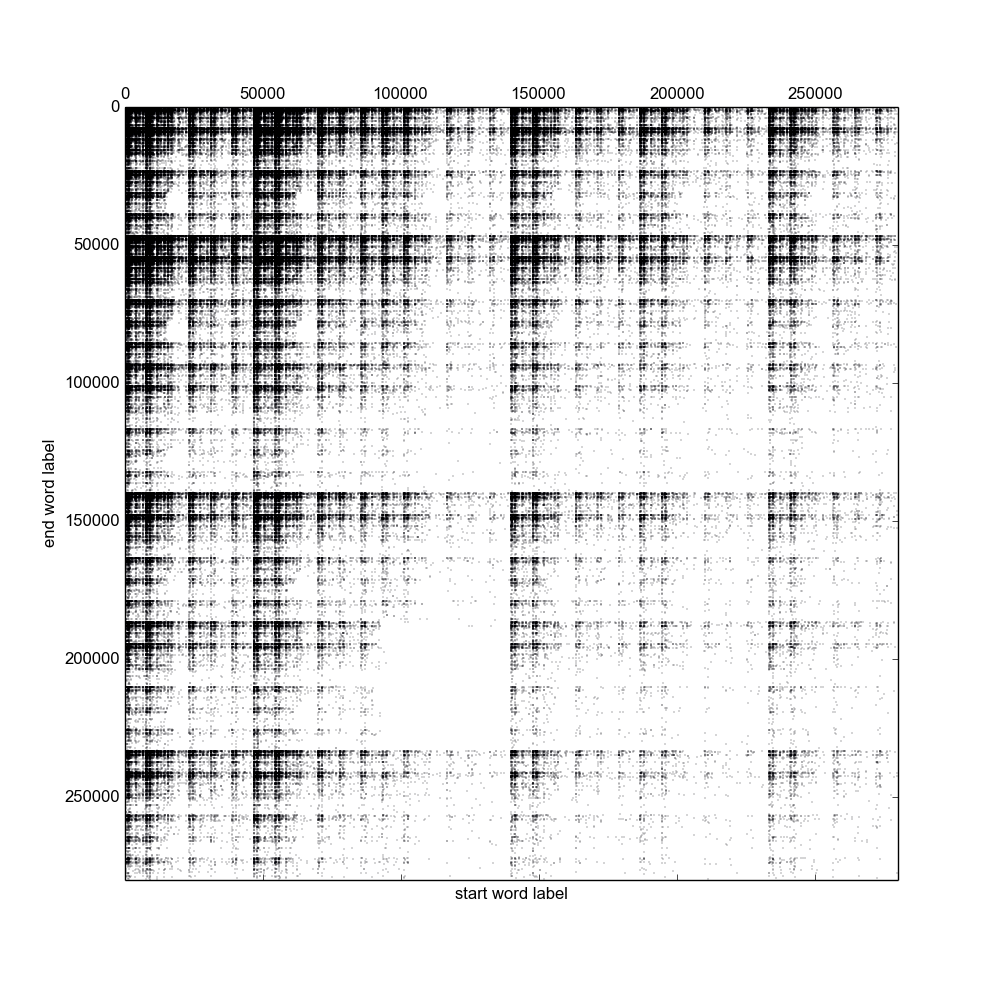
\includegraphics[width=0.45\textwidth]{kronfit6_sparsematplot.png}
  \caption{clockwise from top left: matrix plot(dots are edges) of bigram, matrix plot of \frac{1}{5} of bigram, 6 by 6 Kronecker fit graph, 2 by 2 Kronecker fit graph}
\end{figure}

\begin{thebibliography}{99}
  \bibitem{smallworldlang}
    Cancho, RF. and RV Sole. 2001. "The Small World of Human Language". Proceedings of the Royal Society B: Biological Sciences.
  \bibitem{kronfit}
    Lekovec, J., and Faloutsos, C. 2007. "Scalable Modeling of Real Graphs Using Kronecker Multiplication." Proceedings of ICML.
  \bibitem{mejpowerlaw}
    Newman, MEJ. 2005. "Power laws, Pareto distributions and Zipf's law." Contemporary Physics.
  \bibitem{fractaldim}
    Mandelbrot, BB., 1982. "The Fractal Geometry of Nature." WH Freeman and Company.
  \bibitem{lacunarity}
    Mandelbrot, BB., 1995. "Measures of Fractal Lacunarity: Minkowski Content and Alternatives". Fractal Geometry and Stochastics.
  \bibitem{nltk}
    Bird, S., E. Loper and E. Klein. 2009. "Natural Language Processing with Python." O'Reilly Media Inc.
  \bibitem{richter}
    Stix, G. 1992. "Finding Fault." Scientific American.
  \bibitem{fractalcutoffs}
    Malcai, O., DA. Lidar, O. Biham and D. Avnir. 1998. "Scaling Range and Cutoffs in Empirical Fractals". Physical Review.
  \bibitem{netvalskew}
    Chakrabarti, D., Y. Zhan and C. Faloutsos. 2004. "R-mat: A recursive model for graph mining." SIAM Conference on Data Mining.
  \bibitem{densificationpowerlaw}
    Leskovec, J., JM Kleinberg and C. Faloutsos. 2007. "Graph evolution: Densification and shrinking diameters." ACM TKDD.
  \bibitem{stochkrongraph}
    Mahdian, M., and Y. Xu. 2007. "Stochastic Kronecker Graphs." Workshop on Algorithms and Models for the Web Graph.
  \bibitem{mlcompression}
    Frank, E., C. Chui and IH. Witten. 2000. "Text Categorization using Compression Models." IEEE Data Compression.
  \bibitem{cosma}
    Clauset, A., CR Shalizi and MEJ Newman. 2009. "Power-law distributions in empirical data." SIAM Review.
  \bibitem{gamiller}
    Miller, GA. 1957. "Some Effects of Intermittent Silence". The American Journal of Psychology.
  \bibitem{shannon}
    Shannon, C. E., 1950. "Prediction and Entropy of Printed English". Bell System Technical Journal.
  \bibitem{nltk}
    Bird, Steven, Edward Loper and Ewan Klein, 2009. "Natural Language Processing with Python." O'Reilly Media Inc.
  \bibitem{collins}
    Collins, Michael. 2011. "Tagging with Hidden Markov Models".
\end{thebibliography}


\end{document}
